%
%
%
\documentclass[oneside]{book}


\usepackage{times} 
\usepackage{graphicx} 
\usepackage{xspace}
\usepackage{hyperref}
\usepackage[disable]{todonotes}
%
%
%
\usepackage{listings}
\usepackage{caption,subcaption}
\usepackage{cite}


%
\newcommand{\level}{level\xspace}
\newcommand{\levels}{levels\xspace}
\newcommand{\Level}{Level\xspace}
\newcommand{\Levels}{Levels\xspace}
\newcommand{\hcir}{HC IR\xspace}
\newcommand{\llvmir}{LLVM IR\xspace}
\newcommand{\llvm}{LLVM\xspace}
\newcommand{\ciao}{Ciao\xspace}
\newcommand{\ciaopp}{CiaoPP\xspace}
\newcommand{\tool}{tool\xspace}
\newcommand{\tools}{tools\xspace}
\newcommand{\ial}{IAL\xspace}
\newcommand{\frontend}{front end\xspace}
\newcommand{\Frontend}{Front end\xspace}
\newcommand{\isa}{ISA\xspace}
\newcommand\ciaoppCmdLine{\tt ciaopp\_entra}

\newcommand{\true}{\mathsf {true}}
\newcommand{\false}{\mathsf {false}}

\def\ll{[\![}
\def\rr{]\!]}



\linespread{1.2}

%
\newcommand{\token}{true}
%

%
\newcommand{\hastoken}[3]{
\ifthenelse{\equal{\token}{true}}{
\noindent\fbox{{\color{red} \textbf{Has token:}  #1 (deadline #2)}. \textbf{Token order:} #3} 
\medskip
}{}}




%
\newcommand{\demofigpath}{\figpath}
\newcommand{\attachpath}{attachments}
\newcommand{\figpath}{Figs}
%
\newcommand{\internalcomment}[1]{
\begin{small}
\noindent
{\color{red} #1} \ \\
\end{small}
}
%
 
\setcounter{chapter}{2}
\setcounter{secnumdepth}{3}

\date{\today}
\begin{document}

\chapter{Energy-Aware Software Engineering}

\begin{center}
\textrm{Kerstin Eder,  University of Bristol\\John P. Gallagher, Roskilde University}
\end{center}
\vskip 0.5 cm

\noindent
\textrm{Keywords: energy modelling, energy analysis, energy transparency, energy-aware, software engineering.}
\vskip 0.5 cm

Energy-aware software engineering concerns the use of tools and methods to allow energy consumption to be a first-class software design goal. A design goal could be, for instance, to meet stated energy targets such as battery lifetime or power-supply constraints for a given ICT application running on a given hardware platform, or simply to optimise energy efficiency. Very few programmers at present have much idea of how much energy their programs consume, or which parts of a program use the most energy. Therefore energy-related design goals are usually not considered until the programs are deployed; at that point, if energy goals are not reached, it may result in very long expensive re-development cycles.


Although energy is ultimately consumed by physical processes in the hardware, the software controls the hardware and indeed typically causes a great deal of energy waste by inefficient use of the hardware. This waste cannot be recovered by relying on the development of more energy-efficient hardware -- increasing the energy efficiency of the software is an essential part of reducing overall energy consumption \cite{Furber2016}.  
 Energy-awareness for software development thus requires an understanding of the implications for energy consumption of design decisions in the software. In short, there is a need for \emph{energy transparency}: the ability of the software developer to ``see" the program's energy consumption, ideally without actually executing and measuring it.\todo{or, like in EACOF, to just measure it} \todo{J: what is EACOF?}

\paragraph{Chapter outline.}  Section \ref{greenit} presents the background and motivation for energy-aware software engineering. Then  the main scientific and technical foundations that support energy transparency are summarised.  These are \emph{energy modelling} and \emph{static energy analysis}. Energy modelling (Section \ref{sec:energy-models}) concerns building models of software energy consumption at different levels of abstraction, attributing energy consumption at the hardware level to software constructs such as operations, instructions, statements, functions and
procedures.   Energy analysis (Section \ref{sec:energy-analysis}) concerns the estimation, using an energy model, of the energy that would be consumed when running a piece of software, without actually executing it.  This estimate can be parameterised by the input data for the software, or other contextual information. 

Section \ref{inefficiency} contains a summary of the typical sources of energy inefficiency that can be removed when the programmer has relevant information on energy consumption.   Finally, Section \ref{ea-sw-eng} describes how software designers and developers can use energy transparency during the software engineering process, and what kind of activities constitute ``energy-aware software engineering".  For example, the programmer can analyse the program to identify which part of the software consumes most energy, or explore the effect on
energy consumption of different algorithms and data structures.

In contrast to much work on energy efficiency of ICT, this chapter adopts a generic approach, not driven by any particular class of applications, platforms or programming languages. The topic is currently mainly studied in different application contexts such as embedded systems, high-performance systems, mobile systems and so on, rather than as a coherent set of techniques applicable to any software-based system.

\nopagebreak
\section{Energy-aware software engineering and Green IT}
\label{greenit}
Concern over the increasing energy consumption and general environmental impact of ICT systems is growing.  As a part of this,
there has been a growth of interest in the field of \emph{Green IT}  \cite{KrauseCraigWood2010,DBLP:journals/stt/NaumannKD13,DBLP:journals/infsof/CapraFS12,Mahmoud_Ahmad_2013} since approximately 2010; for example the conference series International Green And Sustainable Computing Conference\footnote{\texttt{http://igsc.eecs.wsu.edu/} (formerly International Green Computing Conference (IGCC))} started in 2011 and the IEEE technical area of Green Computing\footnote{\texttt{http://sameekhan.org/tagc/}} was launched in 2010.  The Energy Aware COmputing workshop series\footnote{\texttt{http://www.cs.bris.ac.uk/Research/eaco/}} was initiated in Bristol in 2011.
More recently, dedicated workshops such as GREENS\footnote{\texttt{http://greens.cs.vu.nl/}} and SMARTGREENS\footnote{\texttt{http://www.smartgreens.org/}} have been launched. 

Green IT covers energy aspects of the complete life-cycle and context of ICT systems, including software and hardware, development energy costs, maintenance and deployment energy costs, cooling costs, the energy costs of communication infrastructure, raw materials and disposal costs and a host of other energy costs and environmental effects associated directly or indirectly with software systems. 



Energy-aware software development is therefore only one aspect of Green IT;  it is only concerned with the energy efficiency of software, that is, the energy costs directly attributable to how programs use the hardware during execution. The energy-aware software engineer cannot in general be aware of the whole Green IT field, which involves complex dependencies and tradeoffs and goes well beyond software engineering.



\paragraph{Environmental motivation.}
The energy consumed by ICT is growing both in absolute terms and as a proportion of the global energy consumption and thus plays an important role in meeting the targets of the Europe 2020 Agenda, which includes a goal to reduce greenhouse gas emissions by at least 20\% compared to 1990 levels.   Every device, from autonomous sensor systems operating at the mW level to high performance computing (HPC) systems and data centres requiring tens of MWs for operation, consumes a certain amount of energy which results in the emission of CO$_2$. 

As already pointed out, energy is consumed by hardware, but the software often causes a great deal of energy waste by inefficient use of the hardware.  Increasing the energy efficiency of the software is at least as effective as development of more energy-efficient hardware.
Furber remarks 
that ``if you want an ultimate low-power system, then you have to worry about
energy usage at every level in the system design" \cite{Furber2016}.
Furthermore, in many cases the energy efficiency of software has a direct positive effect on the efficiency of other energy-related aspects of systems.  Obvious cases are cooling costs and battery costs -- cooling requirements for data centres are directly related to the power dissipated by the computations, while for mobile systems the number of battery replacements or recharges is similarly reduced if software is more energy-efficient.  

\paragraph{Strategic motivation.} 
The energy efficiency of ICT systems plays a critical role in exploiting the massive amounts of information available in data centres, and the full vision of the so-called Internet of Things.  The power requirement of a data centre is typically measured in tens of MW, including cooling costs, while the Internet of Things generates increasing demand for a huge number of very low-power devices. The dream of ``wireless sensors everywhere" is accompanied by the nightmare of battery replacement and disposal unless the energy requirements of software running on devices can be lowered to enable them to be powered by energy harvesters or RF power sources.\todo{should we mention the initiatives by the EC and local governments as well as the US (PERFECT)?} \todo{J: feel free to mention these}

\paragraph{Development costs of energy-efficient software.} In the current state of the art, development costs for energy-efficient systems are higher than for energy-wasteful systems due to the extra effort required to take energy consumption into account. This is a significant barrier to making energy efficiency a first-class design goal.



The motivations for research in energy-aware software development can thus be summarised as follows.
\begin{enumerate}
\item
To lower the energy costs directly attributable to software execution, helping to reduce the environmental impact of ICT and to enable the next generation of ambient low-power devices.
\item
To lower  energy costs indirectly caused by software, such as the cost of cooling, power supplies, battery replacement and recharging.
\item
To reduce the costs of the process of developing energy-efficient systems, by developing tools and techniques to assist the energy-aware developer.
\end{enumerate}

%
\nopagebreak
\section{Energy Modelling}\label{sec:energy-models}

%

An energy model supporting 
%
software energy analysis 
%
associates energy 
consumption costs
with 
basic
program constructs such as source code blocks, basic blocks in the intermediate representation 
%
used during compilation or machine code instructions.
%
In addition, other costs arising from the execution of a program may need to be considered, depending on the micro architectural features of the hardware; examples are costs associated with the memory hierarchy, such as the cost of a cache hit and miss or the cost of accessing on-chip and off-chip memory, and also costs associated with the processor pipeline, such as the cost of pipeline stalls. In addition, the cost of the processor being idle and the cost of processing multiple threads concurrently may also need to be considered. 

An energy model, as understood in this chapter, is program-independent.  It captures the energy costs of basic software constructs in a given language executed on a given hardware platform. The model is used during program analysis (Section \ref{sec:energy-analysis}) to obtain information about the energy consumption of a given program.
%
%

The challenge in energy modelling for software energy analysis is in finding a good compromise between the accuracy of the model and the ease with which the information can be mapped onto software constructs. Regarding the former, model accuracy tends to be higher for models at the lower-levels of abstraction, i.e.\ instruction-level energy models are typically more accurate than energy models at the intermediate representation of the compiler, and source code energy models are less accurate in comparison. 
%
However, understanding which source code lines or blocks consume most energy is much more useful to software developers looking to optimise their code for energy efficiency, than knowing the energy consumed by the sequence of machine instructions issued by the compiler. The higher the level of abstraction at which the information is presented to the software developer, the easier it is for them to comprehend the impact of algorithms and coding on the energy consumed during program execution. Yet, taking measurements to characterise energy models is simplest and most accurate when performed at the lower levels of abstraction, where energy costs of low-level software constructs such as machine instructions can be determined directly.



\subsection{Defining and constructing an energy model at ISA level}\label{subsec:isa}

The Instruction Set Architecture (ISA) is the interface between hardware and
software. 
%
It defines the hardware architecture and its behaviour in terms of low-level
programming constructs such as supported data types, machine instructions,
registers, the memory architecture, any interrupt and exception handling as
well as I/O operations.
%
The ISA provides a practical level of abstraction for energy modelling, because
it is possible to directly correlate the energy consumption of the hardware
operations associated with instruction execution to low-level software
constructs.

Energy modelling at ISA level dates back to 1994 when Tiwari et
al.~\cite{Tiwari-embedded-1994} first proposed a
%
method to develop instruction-level power models for arbitrary
processor architectures to estimate the power consumption caused by software.
%
Such models could overcome the limitations of hardware design power analysis
methods, which require access to gate level design information including layout
and tend to be impractically slow at producing results for system-level power
analysis. Instruction-level power models, instead, are orders of magnitude
faster at estimating the power consumption of embedded software and can achieve
accuracy within 10\% of what hardware design power analysis methods deliver.
This is a worthwhile tradeoff because software development involves numerous
iterations during the coding phase, and rapid feedback of resource usage is
critical for software developers to make energy aware decisions.

The model in reference~\cite{Tiwari-embedded-1994} captures the energy consumption
directly associated with processing each instruction, obtained by measuring the
average current drawn while executing a dedicated loop that only contains
independent instances of the respective instruction to be profiled, multiplied
by the supply voltage $V_{CC}$, and further multiplied by the number and
duration of the clock cycles required to execute the instruction.
%
Variations in instruction base costs can be observed during measurements and
are due to different operand values being used during execution. It was observed that
different operand registers lead to negligible variation, while using different
immediate values or different memory addresses leads to observable, yet small
variation of no more than 5\% for the architectures analysed.
%
Because the exact operand values for instructions are only known at runtime,
the energy model associates a single base cost with each instruction,
representing averaged values. This is a very important feature of a single
instruction cost Tiwari-style energy model as it has implications on the safety
of the bounds inferred by worst case static analysis techniques. This will be
discussed further in Section~\ref{subsec:data}.

Instruction base costs intentionally do not include any extra costs arising
from executing an instruction within the context of other instructions, i.e.\
the overheads of executing arbitrary instruction sequences.
%
One such cost is associated with switching the circuit state from executing one
instruction to executing the next, termed the circuit state overhead. It
captures the extra energy consumed due to switching on busses, e.g.\ as a
consequence of changing op-codes and operand values, and using different
functional units within the processor. The circuit state overhead is determined
for all pairs of instructions by measuring loops that contain alternating
sequences of the two instructions per pair.
%
While including circuit state overheads into the energy model improves the
accuracy of the model, the variation observed for individual instruction pairs
was very limited for the architectures considered. It may thus be sufficient to
determine a constant circuit state overhead cost and to use that instead of
profiling all instruction pairs.

The execution of instruction sequences may give rise to other costs beyond the
cost of circuit state switching, depending on the micro architecture of the
processor. Resource contention due to data dependencies between instructions
may cause pipeline stalls. Thus, the cost of pipeline stalls needs to be
determined together with the number of stall cycles.
%
In addition, there may be costs associated with cache misses, which typically
cause execution delays of varying durations, depending on whether the fetch is
from other cache levels of main memory. Their energy consumption also needs to
be accounted for in an energy model, potentially sourcing information from a
cache model that can provide cache miss rates for a given program. 
%
Thus, while instruction-level energy modelling techniques can be very accurate
for simple architectures, the presence of complex architectural and micro
architectural features such as several layers of caches, pipelines, superscalar
processing, speculative execution etc, can make it very difficult to achieve
acceptable levels of accuracy when modelling at the instruction level.

In~\cite{TiwariWolfeInstructionLevelPowerAnalysi:1996} this energy model is
used to derive the energy consumption of a program $Prog$ by 
 by Equation~\ref{e:tiwari}.
%
\begin{equation}\label{e:tiwari}
E_{Prog} = \sum_i (B_i \times N_i) + \sum_{i,j} (O_{i,j} \times N_{i,j}) + \sum_k E_k
\end{equation}

According to Equation~\ref{e:tiwari}, the energy consumption of $Prog$, namely $E_{Prog}$, is
calculated as the sum of three components: the base cost
of instruction
execution, the
circuit state overhead, and other inter instruction effects.
%
The first term in the sum in Equation~\ref{e:tiwari} represents the base cost, where $B_i$ is
the base cost of instruction $i$ multiplied with the number of times $i$ occurs
in program $\mathit{Prog}$, $N_i$.
%
The second term is the circuit state overhead, where $O_{i,j}$ represents the
cost incurred by switching the circuit state of the processor from executing
instruction $i$ to executing instruction $j$. This is multiplied by the number of
times instruction $i$ is followed by instruction $j$ in program $\mathit{Prog}$, $N_{i,j}$. 
%
Finally, the third term in the sum accounts for the cost of $k$ inter-instruction
effects that may impact on software related energy consumption, e.g.\ cache
misses or pipeline stalls that can be characterised using external cache models
or models of the micro architecture of the processor.

Equation~\ref{e:tiwari} shows clearly the relation between the energy model and the
analysis of the program.  The terms $B_i$, $O_{i,j}$ and $E_k$ are obtained from the energy
model, and are program independent. The terms $N_i$ and $N_{i,j}$ are obtained by
analysis of the program, either dynamically, by profiling and counting the number of 
times each instruction or pair of instructions is executed, or statically as will be seen
in Section \ref{sec:energy-analysis}.

\todo[inline]{Maybe include Steinke / Sarta model that have far more detail - neither is useful for static analysis though.}

Recently, instruction-level energy models have been developed for modern
processors such as the Intel Xeon Phi, a many integrated core architecture for
high-performance computing, and the hardware multi-threaded XMOS XCore embedded
microprocessor~\cite{XMOS:Arch}.

The XMOS XCore instruction-level energy
model~\cite{DBLP:journals/tecs/KerrisonE15} is based on the original model by
Tiwari et al. However, it re-defines the notion of base cost to be the power
dissipated while the processor is idle, and uses individual instruction costs,
scaled by the level of concurrency in the processor's pipeline as well as a
constant overhead to account for circuit state switching between instructions.
%
Model characterisation was performed using a measurement setup and instruction
loops similar to those originally proposed in reference~\cite{Tiwari-embedded-1994}. The
individual instruction costs represent averages over measurements obtained from
running loops with instructions using operands that were generated
pseudo-randomly, constraining values to those valid for the respective
instruction.
%
Evaluation of this multi-threaded instruction-level model showed average error
margins of less than 7\%. \todo{should say how this evaluation was done - with ISS, then move to SA}
%
%
%
However, the model was designed to be used for static energy consumption analysis,
requiring static analysis techniques to determine the number of idle cycles and
the level of concurrent thread activity, in addition to the standard
instruction stream statistics.

In contrast, the Xeon Phi instruction-level energy model~\cite{phimodel} relies
on performance counter statistics that are obtained at runtime, rather than
through static analysis at compile time. This model is designed to be used with
software profiling tools to support energy efficient software development. The
model is built by characterising the Energy per Instruction (EPI) of selected
instruction types using microbenchmarks executed on different processor
configurations in terms of numbers of cores and threads per core. Instructions
are classified in terms of op-code and operand locations, both of which
influence the EPI.
%
The energy consumption of a given workload can then be determined by
multiplying the runtime instruction statistics with the respective EPIs.
%
This model achieves an average error rate of less than 5\%.


Energy modelling at the ISA level gives us the following benefits: energy
costs can be assigned at the instruction level; the same level as is output by
the compiler; there are strong correlations between instruction properties and
energy consumption, for example the number of operands used in the instruction;
and machine instructions can be related back to the original programming
statements written by the software developer, as well as to various
intermediate representations. 

The construction of an energy model at the ISA level also has to address several
challenges.
%
Measurements need to be taken to determine both the base cost for each
instruction and also the circuit state overhead. To achieve this, instructions
are placed into infinite loops, i.e.\ loops of single instructions to obtain
that instruction's base costs or loops of alternating instructions to
characterise pair-wise circuit state overhead. The average current is measured
while the loop is executed. Care needs to be taken to ensure the loop runs for
a sufficiently long time to minimise measurement errors due to loop overheads.
%
However, typically not all instructions can be directly profiled, requiring
indirect or statistical approaches to their characterisation.

In general, for a modern processor with hundreds of instructions the
characterisation of the entire ISA is a significant effort.
%
To reduce the measurement effort, rather than determining a base cost for each
instruction, it may be sufficient to group instructions into classes of similar
energy cost and to determine a single instruction class base cost. Likewise,
instead of measuring circuit state overheads for individual instruction pairs,
a cost that represents switching between instruction classes, or a single
constant circuit state overhead may be sufficient.

In addition, other properties such as the cost of running multiple threads and
the cost of idle periods must be determined for multi-threaded architectures,
and communication costs must be considered for interacting multi-threaded
programs running on multi-core platforms. 
%
%
%
%
%
 

\subsection{Energy modelling at higher levels of software abstraction}
\label{subsec:mapping}

Instruction-level energy models are 
%
useful 
due to the close, almost direct
link of measurements to programming constructs within the ISA. Energy models at
higher levels of abstraction, however, provide more intuitive feedback to
software and tool developers, 
%
albeit 
at the cost of accuracy of the
predictions. 

Modelling at the level of the Intermediate Representation (IR) used by
compilers can be a useful compromise between the accuracy of a lower-level
(ISA) model and the high-level source code. Since the compiler is a natural
place for optimisation, modelling and predicting the energy consumption at IR
level could therefore enable energy specific optimisations.

IR-level energy models have been built using two distinct techniques. One is
based on statistical methods, the other on mapping a lower-level model, i.e.\
one at ISA level, up to the IR level at compile time; both have been developed
for LLVM IR~\cite{LattnerLLVM2004} in the context of the LLVM
toolchain~\cite{LLVM}.

In reference ~\cite{Brandolese2011} statistical analysis was employed to build an
energy model for LLVM IR for the purpose of fast and accurate early-stage
prediction of the energy consumption of embedded software at the function level
to enable compile-time energy optimisation.
%
Modelling starts with instrumenting and compiling the source code of a large
set of benchmarks into architecture-independent LLVM IR to extract block-level
statistics capturing the structural features of the source code in terms of
LLVM instructions. 
%
Profiling of the LLVM IR basic blocks is then performed on a host computer to
capture their dynamic behaviour in terms of basic block execution counts. 
%
The final step then factors in the timing and energy consumption of the target
architecture. Using native compilation, back-annotation techniques to associate
LLVM IR instructions with target machine instructions and statistical analysis,
the target machine specific costs are associated with the
architecture-independent LLVM IR. This requires a cost model of the instruction
set for the respective target machine, which is assumed to be provided by the
manufacturer. The resulting model can be used to estimate the energy
consumption of code for the target hardware, based solely on its
target-independent LLVM IR.

A 
%
mapping technique that lifts an energy model at ISA level to LLVM IR
level is described in~\cite{DBLP:journals/corr/GeorgiouKE15}. The energy characteristics of LLVM IR
instructions are determined from the costs of the associated machine
instructions based on a mapping that tracks which LLVM IR instructions created
which machine instructions during the lowering phase of compilation, i.e.\
after optimisation passes. 

%
The approach provides on-the-fly LLVM-IR energy characterisation that takes
into consideration the context of instructions since there is no
program-independent mapping between ISA instructions and LLVM instructions.
Strictly speaking,
the energy model is still at the ISA level; a program-dependent mapping is used to
obtain energy costs of LLVM-IR instructions and blocks at compile time.
%
The technique has been used for static energy consumption analysis at the LLVM
IR level in~\cite{DBLP:journals/corr/GeorgiouKE15},~\cite{isa-vs-llvm-fopara} and also
in~\cite{grech15}. The accuracy of energy consumption estimation at LLVM IR
level is typically within 1\% to 3\% of that achieved using ISA-level models.
This indicates excellent potential for exploiting this energy transparency
during code generation.
%
In principle, the same mapping technique may be used to map the energy consumption
of programs to even higher levels, such as source code blocks or functions. 

An alternative approach to building a source-level energy model, used in \cite{LiGallagherMobiquitous2016}
to obtain a source code energy model for Android code, 
is to identify
basic energy-consuming operations from the source code and correlate them to
energy costs by measuring energy consumption in a large number of benchmark programs
and analysing the results using techniques based on regression analysis. The
resulting energy model of the basic operations implicitly includes the effect
of all the layers of the software stack down to the hardware, including
compiled code, virtual machine and operating system layers. The approach is
inherently approximate; nevertheless such an approach may be the only feasible
one in cases where the software stack has many complex layers, rendering a
mapping-based approach difficult or impossible.

\subsection{The impact of data on the energy model}\label{subsec:data}

The classic instruction level energy model as described in
Section~\ref{subsec:isa} does not capture the impact of data on software energy
consumption. For instance, a single energy cost is assigned to each instruction
or instruction type.
%
In practice, however, energy consumption is dependent on the data being
processed and, for simple processors, data can make a significant contribution
to energy consumption.
%
\begin{figure}[h]
    \centering
    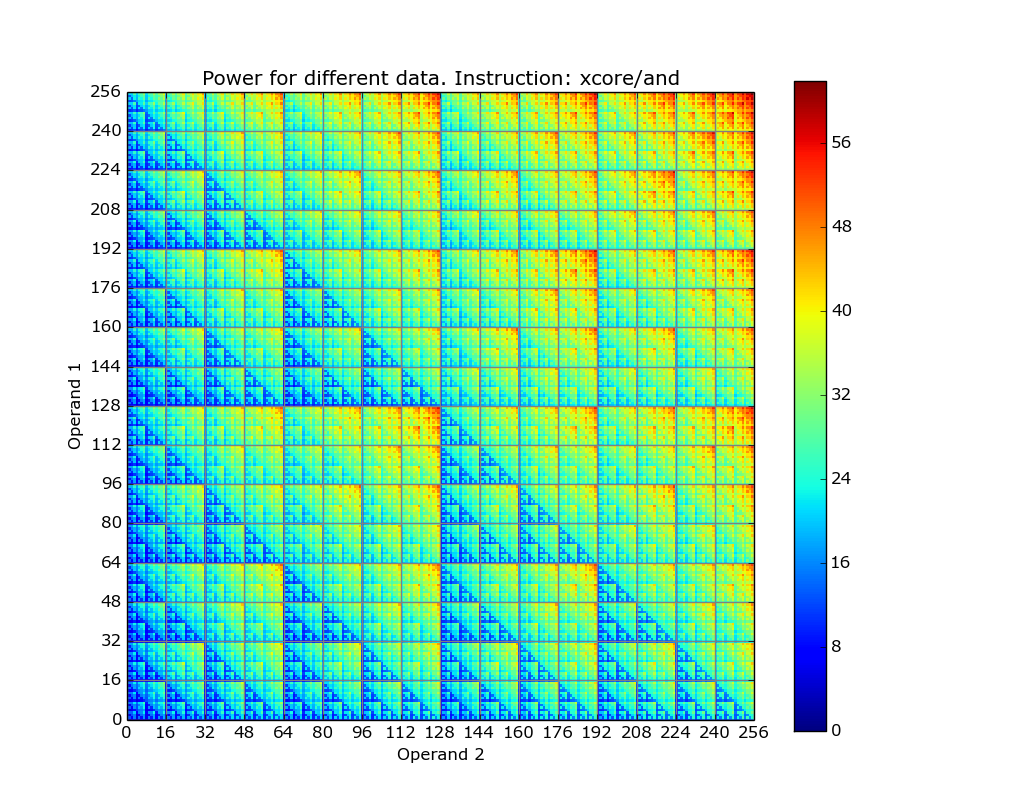
\includegraphics[width = 0.95\linewidth]{Figs/and_map}
    \caption{Dynamic power in mW for the XMOS XCore {\tt and} instruction.}
    \label{f:and-heatmap}
\end{figure}
%
This is illustrated in Figure~\ref{f:and-heatmap}, which shows the dynamic
power, in mW, for the single cycle XMOS XCore bitwise {\tt and} instruction for
all 65536 combinations of 8-bit operands from 0 to 255. The colours in the
``heatmap'' range from dark blue, indicating low power, to dark red, indicating
high power. 
%
In~\cite{DBLP:journals/corr/PallisterKME15} 15\% data induced variation has been reported for
the 8-bit AVR processor, while up to 1.7x data-dependent variation was observed
for the 32-bit XMOS XCore in~\cite{DBLP:journals/tecs/KerrisonE15}. Variation
of as much as 50\% is reported in~\cite{highdatadep} for an ST20 32-bit
microprocessor.

These observations naturally lead to the question of which energy cost should
be associated with an instruction in a single cost instruction-level energy
model. Assigning the averages measured using randomly generated, valid data for
the given instructions is a popular choice. 
%
Estimations based on such models may over- or under-predict the energy
consumption of a program when compared to measurements. Error margins reported
in the literature are typically below 10\%, and over- or under-prediction are
both acceptable when the model is used to obtain estimations of energy
consumption and no guarantees are required.

However, static resource consumption bound analyses must provide bounds on
resource consumption that are both safe and tight, i.e.\ sufficiently close to
the actual values. A good example is Worst Case Execution Time (WCET)
analysis~\cite{DBLP:journals/tecs/WilhelmEEHTWBFHMMPPSS08}, where
under-approximation is not acceptable, i.e.\ unsafe, and significant
over-approximation is considered not useful.
%
Thus, for bound analysis models must support the derivation of safe and tight
bounds. 
%
A key prerequisite to achieve this for WCET analysis is timing predictability
within a system, which enables precise bounds to be established with acceptable
effort, without sacrificing performance of the computation in the general case.
In fact, the architecture of processors can significantly impact on the design
of analysis tools and the properties of the analysis results these can
deliver~\cite{influence-wilhelm-2003} in terms of safety and precision. This is
equally important for static energy consumption analysis, i.e.\ predictable
architectures enable precise models to be developed.

It may be tempting to assign to an instruction the lowest or highest values
observed during measurements to support best and worst case analyses,
respectively. However, this approach has been shown to lead to high
over-approximation~\cite{Wagemann-2015-WCEC} in worst case energy consumption
static analysis, so this may not be a suitable option.
%
In fact, the estimations based on such models may never be reachable in
practice. Intuitively, this is because the data that causes the highest energy
consumption for one instruction is very unlikely to produce output that will
trigger the highest energy consumption also in subsequent instructions. 
%

This leads us to the question of which input data causes the worst energy
consumption for a given program. This question is investigated
in~\cite{DBLP:journals/corr/MorseKE16}, where the problem of data-dependent energy
consumption during program execution is formalised in terms of circuit
switching and a formal proof is presented demonstrating that in general
analysing switching in processor datapaths is NP-hard. Thus, 
%
optimal
data-sensitive worst case energy consumption analysis of programs is, in
general, not achievable efficiently and alternative approaches 
giving good approximations
must be
developed. This is an area of ongoing research.

In~\cite{DBLP:journals/corr/PallisterKME15} energy modelling for worst case energy consumption
analysis has been explored. The most promising approach uses probabilistic
energy distributions to characterise individual instruction pairs and proposes
techniques to compose these to block-level instruction sequences.
%
In~\cite{highdatadep} activity indices were introduced into a single cost
instruction-level model to achieve higher precision of energy consumption
predictions and to enable bound analysis for architectures where data
significantly impacts on energy consumption.

\todo[inline]{Should there be a ``summary'' at the end?}

 
%

\section{Static Analysis of Energy Consumption}\label{sec:energy-analysis}

Static analysis is the other key component of energy transparency.
Given an energy model assigning energy costs to some basic units of the program,
the task of analysis is to determine the overall energy consumption of the program, or
the distribution of energy consumption over the parts of the program.
Static analysis infers information about energy consumed by programs without
actually running them, in contrast to dynamic analysis, which collects information
about the program's behaviour while executing it.  Here we consider only static analysis.

As with energy modelling, analysis can be performed on
program representations at different levels 
in the software stack, ranging from source code (in different programming
languages) through intermediate compiler representations down to ISA level, and employing
an appropriate energy model at that level.



\begin{figure}
  \begin{subfigure}[b]{.49\linewidth}
  \centering
         \begin{lstlisting}
    1: void f(int n) {
          z = 1;
    2:    while (n > 0) {
             z = z*n;
             n = n-1;
    3:    }
          print(z);	
    4: }		
              \end{lstlisting}
    \caption{}
  \end{subfigure}
  \hspace{0.5cm}
  \begin{subfigure}[b]{.49\linewidth}
\begin{center}
\[
     \begin{array}{l}
	true \rightarrow r_1(n)\\
	(r_1(n) \wedge z=1)  \rightarrow r_2(n,z)\\
        (r_2(n,z)~ \wedge \\
	n < 0 \wedge z'=z*n  \wedge n'=n-1)\\
         \ \ \       \rightarrow r_3(n',z')\\
        (r_3(n',z') \wedge n=n' \wedge z=z')\\
        \ \ \         \rightarrow r_2(n,z)\\
        (r_2(n,z) \wedge n \ge 0 \wedge print(z))\\
         \ \ \      \rightarrow r_4	
     \end{array}
\]
    \end{center}
    \caption{}
  \end{subfigure}\\ \\
    \begin{subfigure}[b]{\linewidth}
\begin{center}
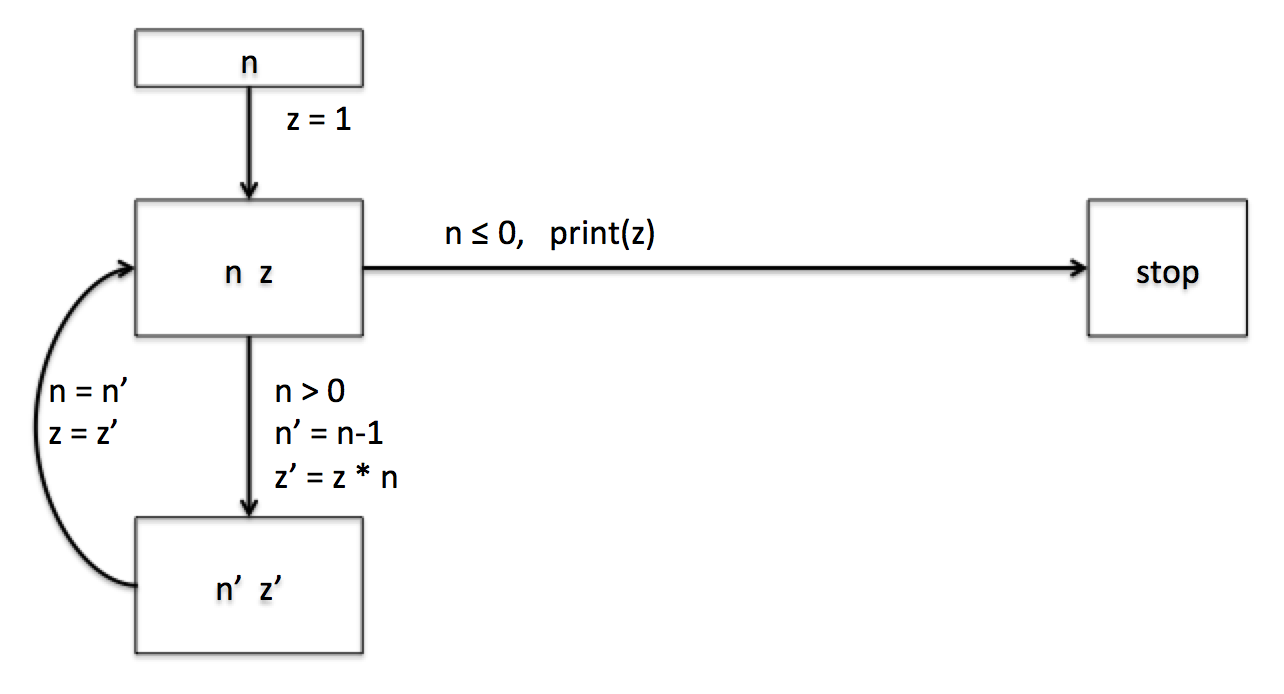
\includegraphics[width=7cm]{\figpath/transition-system}
    \end{center}
    \caption{}
  \end{subfigure}\\

  \caption{Transition system and constrained Horn clauses representing a program}
  \label{fig-horn}
\end{figure}

\begin{figure}
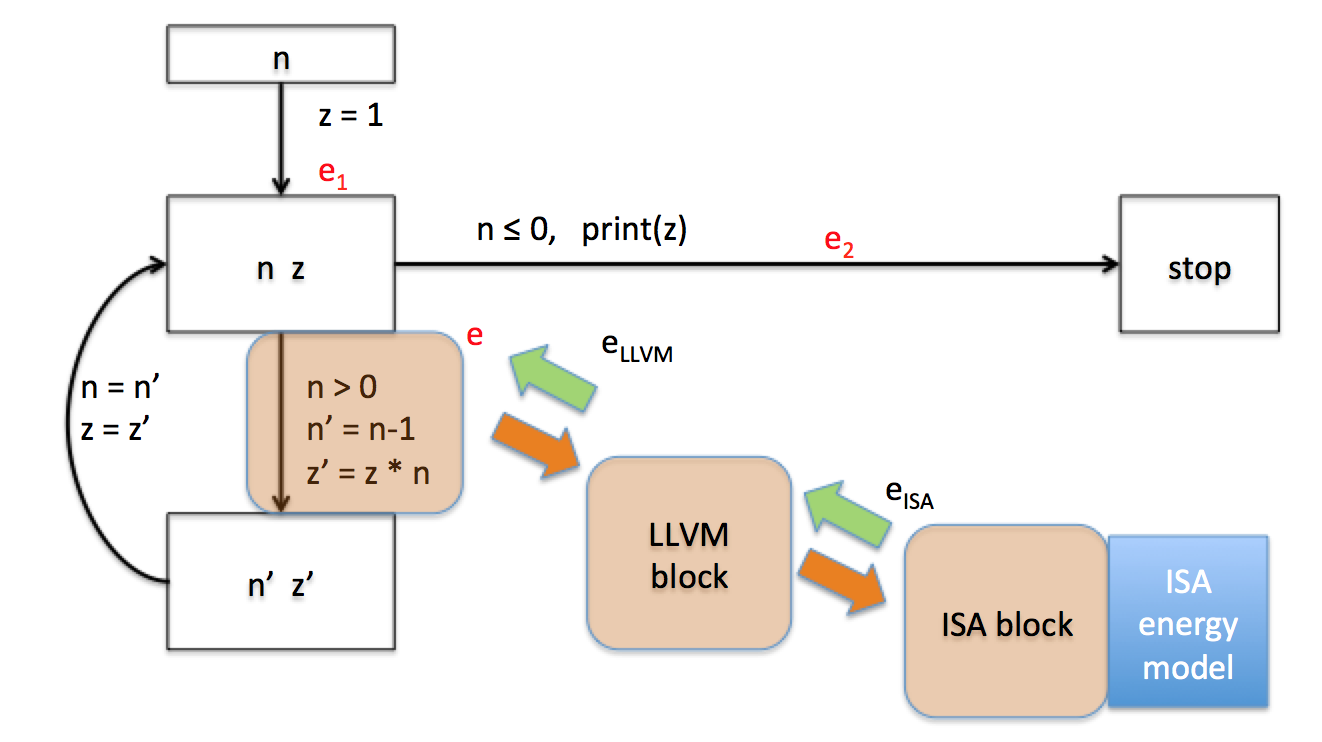
\includegraphics[width=8cm]{\figpath/mapping}   
 \caption{Combining an energy model with program analysis}
 \label{fig-model-mapping}
 \end{figure}

\subsection{Semantic representations of programs}
Static analysis of a program, and in general any formal treatment of programs, requires reference 
to a semantic model of the program derived from the semantics of the
programming language in which it is written. Several different semantic styles
and notations are used, including denotational semantic, small-step or structured
operational semantics, and big-step or natural operational semantics.
All of these can be applied to code
 at various levels such as source code, intermediate compiler
representations or ISA.

A common representation language, suitable mainly for operational semantics, is
constrained Horn clauses (CHCs), a subset of first order logic which is
widely used in software verification
\cite{DBLP:conf/birthday/BjornerGMR15}. CHCs can represent code semantics at any
level of abstraction. In this section we outline the key aspects of
resource analysis using CHCs as a representation, but space does not
allow a fully detailed presentation.  More information can be found in the
references given in the text.

A constrained Horn clause has the form $\forall x_0 \ldots x_n 
(p_1(x_1) \wedge \ldots \wedge p_n(x_N) \wedge \phi \rightarrow
p_0(x_0))$. When representing program semantics, each predicate
$p_0,p_1,\ldots,p_n$ typically corresponds to a program point, and its
respective arguments $x_0,x_1,\ldots,x_n$ are tuples representing the
state before and/or after those points.  A clause thus represents a
relationship between program states, and the constraint $\phi$ expresses
the relationship between the values of the state variables. A special case
of a Horn clause is where $n \le 1$, that is, there is at most one atomic
formula on the left of the clause.  Such a clause often represents a transition 
from the state at one program point to the next.

Figure \ref{fig-horn} illustrates the use of Horn clauses to 
represent an imperative program in a C-like language (a).
The constrained Horn clauses (b) represent a transition
system (c) induced by the program's small-step operational 
semantics (the quantifiers in
the Horn clauses are
omitted).  The predicates
$r_1, \ldots, r_4$ represent the program points $1,\ldots,4$ and
$r_i(x_i)$ means that program point $i$  is reachable with state
$x_i$, where $x_i$ is the tuple of variables in scope at that point.

Lower-level programs such as ISA or intermediate code can be translated
in a similar fashion, where typically each predicate represents a basic block 
in the code. Examples of the translation of XCore ISA programs
to Horn clauses are given in reference \cite{isa-energy-lopstr13-final}.
Semantics-based methods for translating sequential
imperative programs to
Horn clauses are explained in \cite{DBLP:conf/ppdp/AngelisFPP15}.
Furthermore techniques for representing multi-threaded
code as Horn clauses have been developed \cite{ GrebenshchikovLPR12}.


\subsection{Techniques for energy analysis}

Given such a representation of a program, techniques based on abstract interpretation \cite{Cousot1977}
can derive safe approximations of program behaviour.
In terms of CHCs, abstract interpretation can yield
safe approximations of the values of the arguments of each predicate, which represents the
set of possible
states at some program point.
A branch of abstract interpretation 
focusses on automatic complexity analysis, yielding complexity functions on the
execution time of the program \cite{DBLP:journals/cacm/Wegbreit75,Rosendahl89,caslog,resource-iclp07,jvm-cost-esop}.  
These techniques have been widely applied to
analysis of Horn clauses, and have been extended to analysis of energy and
other resources \cite{resource-iclp07,jvm-cost-esop}. Tools such as CiaoPP \cite{ciaopp-sas03-journal-scp} 
and COSTA \cite{AlbertAGPZ08b} have inbuilt
facilities for resource analysis of programs including CHCs.

The essence of the techniques is to extract constraints from the Horn clauses
representing the energy consumed. These constraints represent an abstraction of the behaviour
of the program, in which the energy (or other resource being considered)
can be considered as an implicit extra argument in the predicates of the Horn clauses.
(In some approaches, the extra resource arguments are actually inserted into
the Horn clauses, yielding a so-called ``instrumented" representation).
These constraints are then solved, or approximated, to yield explicit 
formulas giving the consumption.


 
\paragraph{Linking analysis to an energy model.} The Horn clauses in the semantic
representation can be 
associated with energy values, using an energy model. For example, if the clauses are obtained
from the source code, then each clause represents the execution of one statement or
source code expression, and a corresponding source code energy model is associated with
that clause.
If the clauses are obtained from lower-level code such as ISA, a clause typically represents 
the execution of
an instruction or basic block;  the corresponding energy consumption from the model can be
mapped to the clause. The energy from a lower-level model
such as an ISA model can also be mapped to a Horn clause representing 
a higher-level construct, possibly via an intermediate level as indicated in Figure \ref{fig-model-mapping}. 

Once this is done, constraints
representing the energy consumption of the program are extracted from the Horn clause 
representation. To make the explanation more intuitive, we explain the process in terms of the transition system,
rather than the Horn clause representation. In the case of the loop at point 2, a recursive equation is obtained, e.g.
\[ cost_2(n) = e + cost_2(n-1)~ (\mathrm{if}~n > 0), ~~cost_2(n) = 0 ~ (\mathrm{if}~n \le 0) \]
where $e$ is the energy cost of one iteration of the loop, obtained from the energy model. A dependency analysis
also determines that the variable $n$ is the relevant input parameter in this case. These
equations can be solved to yield the expression giving the cost of the loop as a function of $n$, 
namely $cost_2(n) = n*e$, and the cost of the whole 
program (a path from 1 to 4) is $cost(n) = e_1 + n*e + e_2$, where $e_1, e_2$ are the respective
energy costs of the transitions before and after the loop.

\paragraph{More complex analyses.} The example shown is very simple, but the method generalises to
more complex control and data structures.  
As the data and control-flow analysis of abstract interpretation is inherently approximate, 
the analysis in general gives safe upper and lower bounds on the 
number of times each part of the program is executed. This in turn gives upper and lower bounds on the energy
consumed by the program.  However, recall that the upper and lower bounds are also relative to the energy model,
as discussed in Section \ref{subsec:data}. If the energy model supplies average costs for the basic instructions
or operations, then the upper and lower bounds on the energy given by the analysis might not be safe, since the
actual costs of executing the instructions might be respectively higher or lower than the average.

A further extension of the method of generating constraints and solving them yields
static energy profiling~\cite{staticprofiling-flops}, which shows the
distribution of energy usage over the parts of the code, rather than a single function giving the total consumption of the program.
 
\nopagebreak
\section{Software energy optimisation}
\label{inefficiency}
 
 
One of the first works to stress the general importance of software energy efficiency, and identify  aspects of software that affect energy consumption, was by Roy and Johnson \cite{Roy_Johnson_1997}. More recent software-based approaches to achieving lower energy consumption are covered in \cite{Larsson2011,Steigerwald_Agrawal_2011}. 



\subsection{Computational efficiency}\label{compeff}
Firstly, there is a strong correlation between time and energy consumption for a given platform running a single computation thread. There are two reasons for this: less time means fewer instructions and secondly when the task is finished the processor can revert to a lower-power state for the excess time that a less efficient algorithm would use. The latter is called the ``race to idle" in \cite{Steigerwald_Agrawal_2011}. The correlation between time and energy is especially strong when asymptotic complexity is considered.  It is highly likely, for example, that a single-threaded task that has $O(n^2)$ time consumption also has $O(n^2)$ energy consumption.  Thus one of the main concerns of the energy-aware programmer, even with no knowledge of the energy consumption of the hardware, is to find computationally efficient algorithms and data structures suited to the task at hand.

\subsection{Low-level or intermediate code optimisation}
There is a range of techniques for low-level code energy optimisations, which could in principle be carried out by a compiler.  These range from register allocation policies to avoid overheating a few intensively-used registers, use of VLIW (Very Long Instruction Word) instructions and vectorisation, to exploitation of low-power processor states using frequency and voltage scaling (DVFS).  Note that such optimisations, in contrast to computational efficiency, are highly platform-dependent and rely on a platform energy model expressed at the level of low-level code.  Computational efficiency as described in Section \ref{compeff} is also important  in that low-level code optimisations are most effective when applied to frequently executed sections of code, such as tight inner loops, where a small savings in energy can make a significant different to the overall computation. 

Some energy optimisations rely on advanced compile-time (i.e. static) analysis. For example, knowledge of thread load imbalance and knowledge of predictable idle periods when processors can be put into low-power states are difficult to apply in the current compiler state of the art, since the analyses providing this knowledge are still emerging research areas.


\subsection{Parallelism}

The relationship between computational efficiency, time consumption and energy consumption is more complex for parallel than for sequential code.  A multithreaded solution using multiple cores is often more energy-efficient than a single-threaded solution, even though the total amount of work done is greater for the multithreaded code, due to the extra instructions needed for communication and synchronisation. The savings are mainly due to the fact that the overall task time is reduced, and so the processor(s) can revert sooner to a low-power state (the ``race to idle" mentioned earlier).  

Secondly, there can be energy savings if one or more cores can be run more slowly and still achieve the same overall task time as the sequential code.  This is because power ($P$), frequency ($f$) and voltage ($V$) are related by the equation $P = c V^2 f$ where $c$ is a constant. Thus slowing down the processor (reducing $f$) saves power but not overall energy since the computation time is increased proportionally. However, a lower frequency is typically accompanied by a lower voltage, and the power/energy savings are quadratic in relation to voltage reduction.

\subsection{Data and communication efficiency}

Energy can be saved by minimising data movement. This can be achieved by writing software that reduces data movement by using appropriate data structures, by understanding and exploiting the underlying system's memory hierarchy and by designing multithreaded code that reduces the cost of communication among threads.  

For example the size of blocks read and written to memory and external storage can have a major impact on energy efficiency, while memory layout of compound data structures should match the intended usage in the algorithm, so that consecutively referenced data items are stored adjacently if possible.  In multithreaded code, consolidating all read-writes to or from disk to a single thread can reduce disk contention and consequent disk-head thrashing \cite{Steigerwald_Agrawal_2011}.  Furthermore, knowledge of the relative communication distances for inter-core communication can be used to place frequently communicating threads close to each other \cite{KerrisonSwallow15} thus reducing communication energy costs.

Synchronisation mechanisms can also have a serious impact on energy consumption. Waiting for events using polling loops is a notorious example as pointed out by Furber (``a polling loop [is] just burning power to do nothing") \cite{Furber2016}.





\section{Software Engineering Activities and Scenarios}
\label{ea-sw-eng}


We now look at energy-aware software from the designer's and developer's point of view.
What are the activities that distinguish energy-aware design and development from
standard approaches in which energy is considered at the end of the development process, if at all?
In Section \ref{sweng-activities} we identify a number of generic activities that play an
important role in energy-aware software engineering.  In Section \ref{sweng-scenarios} we make the discussion
a little more concrete by sketching scenarios in which these activities are applied.
\begin{figure}
\centerline{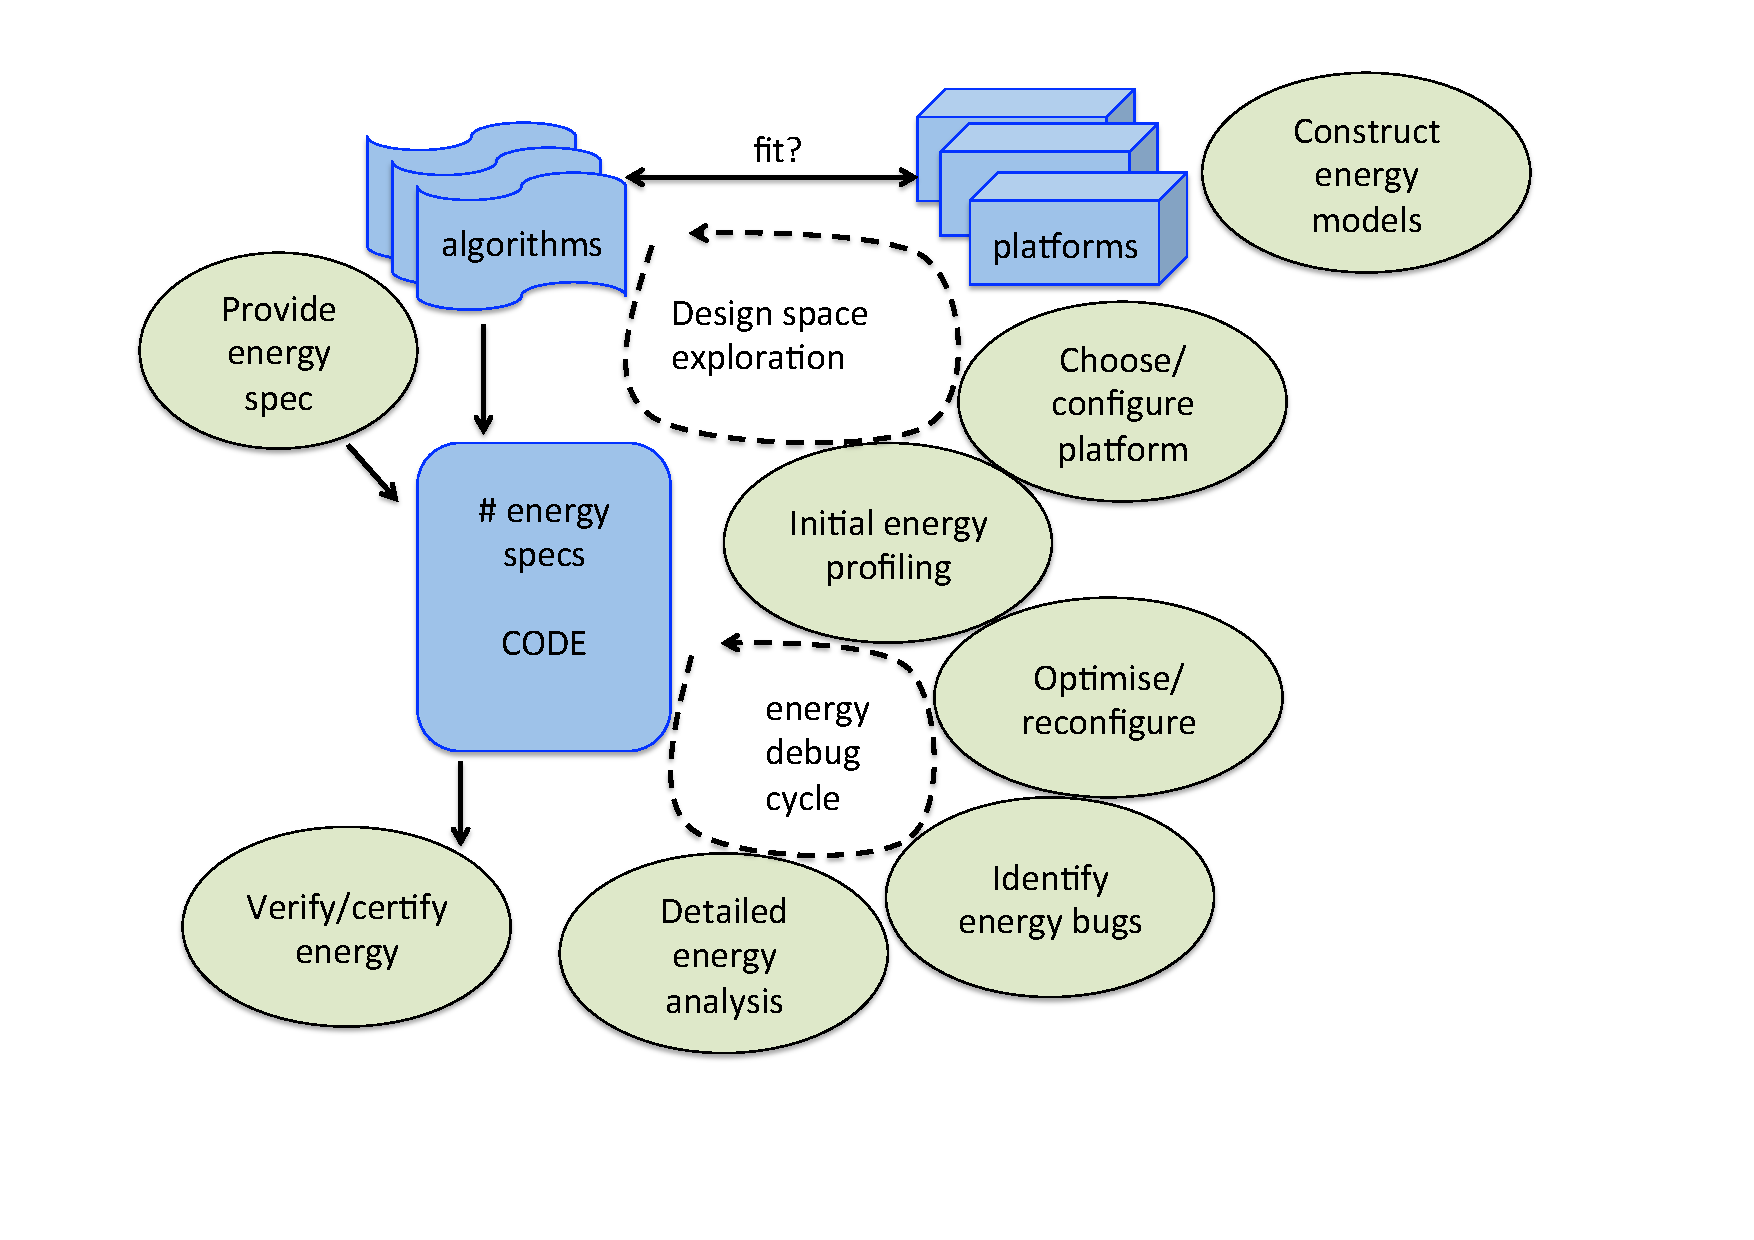
\includegraphics[width=14cm]{\figpath/EASWEngineering-slide}}
\vspace{-1.5cm}
\caption{Energy-aware software engineering activities.}
\label{fig:EASWEngineering}
\end{figure}


\subsection{Energy-aware software engineering activities}\label{sweng-activities}

In this section we describe the most important activities involved in
energy-aware software engineering.  Some of these activities are
extensions or modifications of conventional software engineering
practices; others are new activities that only exist when energy
efficiency is a design goal.  Figure \ref{fig:EASWEngineering} shows a
number of activities and (some of) the inter-dependencies that arise
in the context of different scenarios.

\subsubsection{Specify application, including energy}
The process of developing application software starts with a
requirements specification that expresses not only \emph{functional} properties, as
in the classical approach, but also \emph{non-functional} properties,
including energy consumption and other resources.  Classical
methods for requirements specification need to be extended to allow
non-functional specifications to be expressed. 

Satisfying
functional properties (in the sense of the classical concept of
correctness with respect to a test suite or a formal input-output
specification) is as important as doing so for non-functional
properties: an application that makes a device run out of batteries
before a task is completed is as erroneous and useless as an
application that does not compute the right result. 

\subsubsection{Construction of energy models}\label{energy-models}

Creating energy models for different combinations of hardware platforms and programming 
languages is a part of the energy-aware development process.  At one end of the 
spectrum,  one might
expect future hardware manufacturers to deliver an energy model for their instruction set architecture 
and thus the model would be available ``off the shelf".  At the other end, some
projects might require the construction of an energy model specific to that project, perhaps
because the hardware or software environment was not standard.  In between these two
extremes, energy modelling  for energy-aware software development is becoming a more
well understood process.

\subsubsection{Resource model of deployment platform}\label{platform-model}

If energy efficiency is a design goal, we need to obtain an \emph{energy model
of the platform} on which the system is to be deployed (even though the
software might be developed on a different platform).

Thus obtaining the appropriate energy model is a vital task in energy-aware 
software engineering.  Not only should an appropriate platform be selected, but
its energy model should be available during software development to support other 
activities (see for example Sections \ref{space-expl}, \ref{init-energy}, \ref{energy-analysis} and \ref{energy-bugs}).
We note also that several different energy models for a given platform might be
selected, at different levels of abstraction suitable for different activities.  For instance,
high-level approximate models might be suitable for design space exploration (Section \ref{space-expl}) and initial energy profiling (Section \ref{init-energy}), while more precise low-level models are needed for detailed energy analysis (Section \ref{energy-analysis}) and optimisation 
(Section \ref{energy-opt}).

\subsubsection{Selection of deployment platform}\label{platform-choice}

The choice of deployment platform itself might depend on its resource-usage model; thus 
this activity and Section \ref{platform-model} are interdependent.
By ``platform"
here is meant both the hardware and the software platform; thus the model
should be capable of predicting the energy usage of software (in a given language
and with a given runtime environment) 
being executed on a given piece of hardware.

\subsubsection{Configure platform}\label{platform-config}

Some platforms allow configuration that can have implications for energy consumption.
Among such settings are clock frequency and voltage, the
number of cores and the communication paths among them. At the software level,
operating system settings can also be considered, such as the settings for power saving 
and the resolution of OS
timer processes that can send interrupts to other processes.


\subsubsection{Design space exploration}\label{space-expl}

Choices taken early on in the design process can have a profound effect on the
energy efficiency of the final result.  \emph{Design space exploration} as an 
energy-aware software development activity refers to the process of estimating
energy implications of different possible design solutions, before they are implemented.
It may involve especially activities such as Selection of deployment platform (Section \ref{platform-choice}), Platform configuration (Section \ref{platform-config}) and Initial energy profiling (Section \ref{init-energy}).
This involves energy modelling and analysis tools as in some other activities, but
with the difference that one is likely to be more satisfied with approximate models
and thus rougher estimates
of energy consumption rather than precise predictions.

\subsubsection{Initial energy profiling}\label{init-energy}

At early stages of energy aware software design and implementation, tools are needed 
to perform an \emph{initial energy analysis}.  The purpose
of this is to produce statically an \emph{energy profile} that
identifies the overall
complexity of the energy consumption of the software and how energy consumption is
distributed over the parts of the program.   It could also at this stage identify
energy bugs (parts of the application software that do not meet
their energy consumption specification).

Initial energy analysis requires an
an \emph{energy model} of the deployment platform at an appropriate
level of abstraction. At early stages, parts of the software may be missing
and it might not be possible to compile it to machine instructions; thus
an approximate model based on a model of source code might have to
suffice.

\subsubsection{Detailed energy analysis}\label{energy-analysis}

During more advanced stages of energy aware software implementation,
detailed energy analyses at finer levels of granularity are needed.
These are provided by tools containing more precise low-level energy models 
of the platform, able to give precise estimates of the energy consumption
of critical parts of the code, which could be targets for energy optimisation.  


\subsubsection{Identify energy bugs}\label{energy-bugs}
Energy bugs occur when software does not conform to an energy specification.
The specification might state some overall resource requirement in which
energy consumption is implicit, for example on the length of battery life.  The
bug in such a case could be some energy-consuming process that is more
expensive than necessary, a service that is not switched off when required,
threads that synchronise badly and spend too much time waiting, and so on.


\subsubsection{Energy optimisation or reconfiguring}\label{energy-opt}

The broad concept of energy optimisation is applied throughout the whole software
engineering process, and starts
right at the beginning with design space exploration and selection of appropriate platform,
algorithms and data structures.

The specific energy optimisation performed in this activity 
is driven by the detailed energy analysis
and the energy model of the platform.  Both manual and automatic
optimisations can be applied; the energy analysis should point to the sections of
code that use the most energy, either because they involve costly energy operations,
or because they are frequently executed (e.g., tight inner loops).
This activity also includes application of energy-optimising compilers and such
generic optimisers.

\subsubsection{Verify or certify energy consumption}\label{certify}

Energy-critical applications need to be certified with respect to an
energy specification. Tools combining detailed energy models and
precise energy analysis are required in order to compare the inferred
energy consumption with the specification, either verifying conformance or 
certifying that it holds within some specified limits of behaviour such
as input ranges.


\subsection{Energy-aware software engineering scenarios}\label{sweng-scenarios}


In this section we sketch scenarios in which the activities described
in the previous section are applied.

\subsubsection{Embedded system development on xCORE}\label{xcore-scenario}

The ENTRA project\footnote{\texttt{http://entraproject.eu}} considered energy analysis of embedded systems implemented in the XC language and deployed on the xCORE multicore architecture.  An energy-aware software development strategy for such applications involves the following energy-aware activities.
\begin{itemize}
\item
Energy specification by writing pragma comments in the XC source code.  Such pragmas could express energy constraints derived from customer requirements on the power supply.
\item
Platform selection and configuration.  The xCORE architecture is highly configurable both in terms of the number of cores and their interconnection.  The choice and configuration is guided by an energy model applied to proposed solutions, taking into account thread communication energy costs in a given configuration, as described in more detail in \cite{KerrisonSwallow15}).
\item
Detailed program-independent energy models of the platform at \isa\ level, are available.  
Program-dependent energy models are obtained for XC and \llvmir\ code for the application from the \isa\ model, and used to perform more precise and detailed energy analysis of the application.
\item
Optimisations of expensive or frequently executed code is performed on the basis of the energy analysis.
\item
The energy optimising compiler for XC is applied to the application.
\item
Pragmas in the code are verified using comparison of the energy consumption predicted by the analysis with the constraints in the specification.  

\end{itemize}

\begin{figure*}
	\centering
	\begin{subfigure}[b]{0.49\textwidth}
		\centering            
		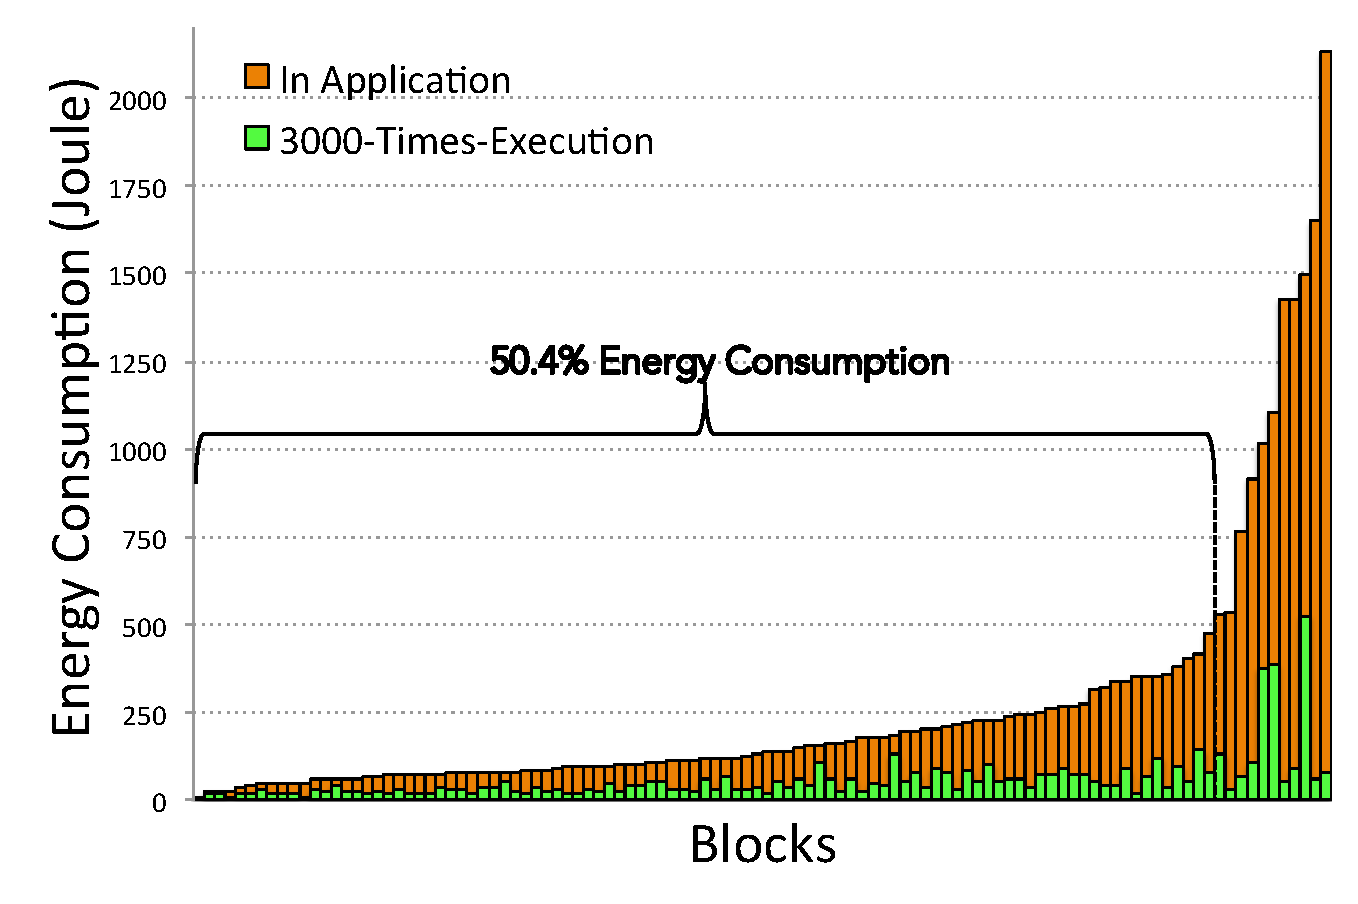
\includegraphics[width = \textwidth]{Figs/blocks_in_program.pdf}
		\caption{ Block costs ``In Application" and in ``3000-Times-Execution".}
		\label{fig:blocks_in_program}
	\end{subfigure}
	%
	%
	\begin{subfigure}[b]{0.49\textwidth}
		\centering
		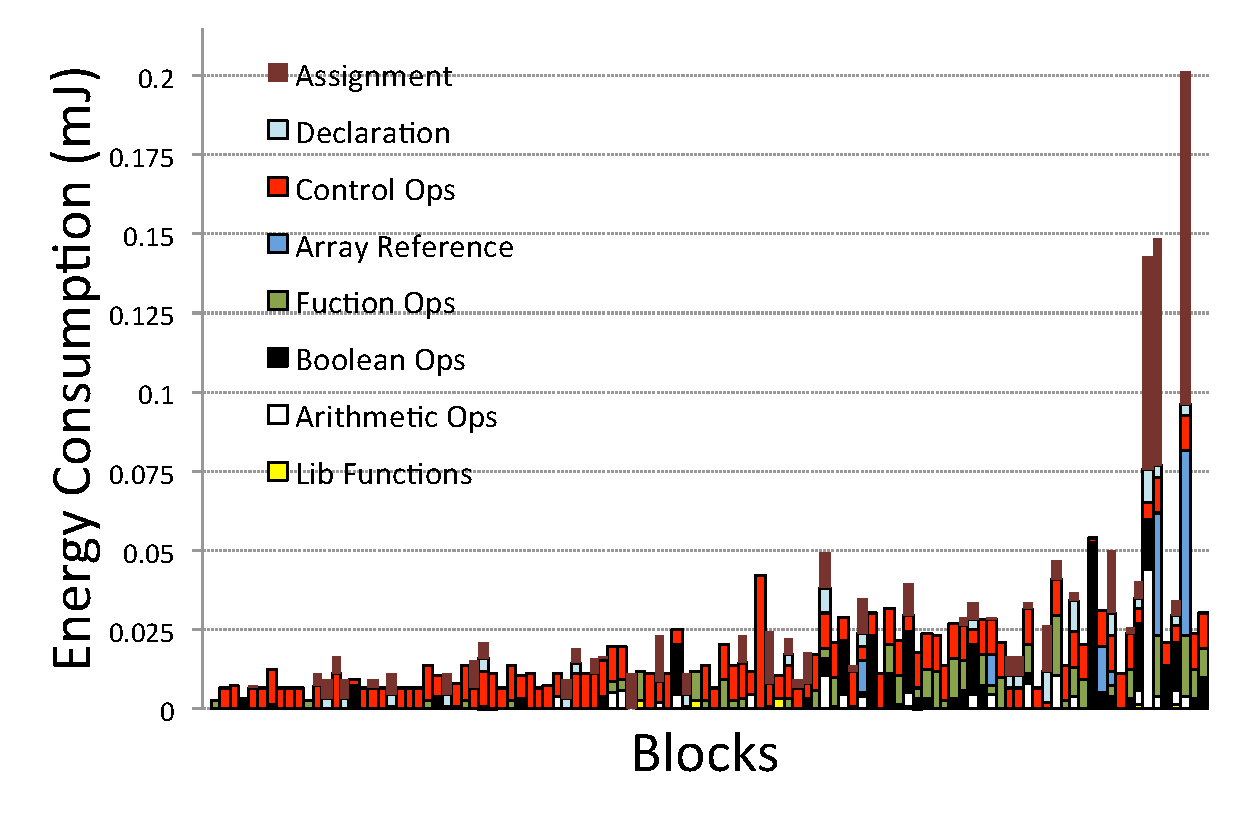
\includegraphics[width=\textwidth]{Figs/op_in_block.pdf}
		\caption{Energy proportions of different kinds of operations in blocks.}
		\label{fig:op_in_block}
	\end{subfigure}
	\caption{Energy distribution over basic blocks in an Android application. Blocks are sorted by the order of their contribution to run-time energy costs. The green bars indicate the relative costs of the blocks.}\label{fig:block}
\end{figure*}

\subsubsection{Android app development}\label{android-scenario}

A case study on Android app energy optimisation was carried out \cite{LiGallagherSCAM2016}.  
The study involved  energy modelling and optimisation of applications based on an established game-engine.  
An energy specification was not given; the aim of the study was to use a source-code-level energy model to 
identify the most energy-intensive parts of the code in a number of typical use-cases, 
and then apply manual optimisations, reducing energy usage directly and thus prolonging battery life.

Energy-aware software engineering activities included:
\begin{itemize}
\item
Building a fine-grained source code energy model by regression
analysis from energy measurements on the target hardware and Android
software platform of a set of test cases exercising the functions of
the underlying game engine.

\item

Dynamic profiling of the code, which provided an energy profile that
allowed the most energy-expensive basic blocks to be identified. For example, Figure \ref{fig:block} 
from \cite{LiGallagherSCAM2016} shows an example of how the relative energy cost of
basic source code blocks enables the programmer to focus optimisation effort on the most energy-consuming
blocks.


\item Manual refactoring of the source code, targeted at the most
  expensive blocks, which succeeded in increasing energy efficient by
  a factor of 6\% to 50\% in various use-case scenarios.
\end{itemize}

\section{Summary}\label{sec:summary}

The purpose of this chapter was to motivate energy-aware software engineering and to outline the principles and methods underlying it.
We discussed why it is worth focussing on energy efficiency during software development, and why energy efficiency should be
a first class software design goal. 

A key concept is energy transparency, which makes the energy consumption of a program explicit at the level of code, rather than at the
level of hardware, where the energy is actually consumed. A substantial part of the chapter described the two
main fields of study relevant to energy transparency, namely energy modelling and static analysis.
Energy transparency is achieved by analysis of a program with respect to
an energy model.  The model associates energy consumption costs with basic units of the software, such as instructions or statements, and
includes also other costs and overheads. Static analysis for energy consumption
 is a semantics-based formal technique, extending methods for automatic complexity analysis of programs,
which is a branch of abstract interpretation.

The last part of the chapter considered the various features of software that can affect energy consumption. An energy-aware developer 
can use energy transparency to focus energy-aware design and optimisation in the most effective way. The field of
energy-aware software engineering is only just emerging, and we described a number of activities that characterise
energy-aware software engineering, extending or modifying conventional practices. The chapter concluded with
a description of two short scenarios of energy-aware software engineering; however
a great deal of further experience and 
tool development is needed to realise the full vision.


\section*{Acknowledgements}

This chapter is largely based on work done in the EU 7th Framework project ENTRA: Whole-Systems ENergy TRAnsparency (318337).
Thanks are due to all the participants in the project, especially Pedro L\'{o}pez Garc\'{i}a, Henk Muller, Steve Kerrison, Kyriakos Georgiou, James Pallister, Jeremy Morse and Xueliang Li 
for material incorporated in the chapter.

\bibliographystyle{unsrt}
%
\begin{thebibliography}{10}

\bibitem{Furber2016}
Steve Furber.
\newblock Interview with {S}teve {F}urber: The designer of the {ARM} chip
  shares lessons on energy-efficient computing.
\newblock {\em ACM Queue}, 8(2), 2016.

\bibitem{KrauseCraigWood2010}
P.J. Krause, K.~Craig-Wood, and N.~Craig-Wood.
\newblock {Green ICT}: {O}xymoron, or call to innovation?
\newblock In {\em Proc. Green IT}, Singapore, 2010.

\bibitem{DBLP:journals/stt/NaumannKD13}
Stefan Naumann, Eva Kern, and Markus Dick.
\newblock Classifying green software engineering - the {GREENSOFT} model.
\newblock {\em Softwaretechnik-Trends}, 33(2), 2013.

\bibitem{DBLP:journals/infsof/CapraFS12}
Eugenio Capra, Chiara Francalanci, and Sandra Slaughter.
\newblock Is software ``green"? {A}pplication development environments and
  energy efficiency in open source applications.
\newblock {\em Information {\&} Software Technology}, 54(1):60--71, 2012.

\bibitem{Mahmoud_Ahmad_2013}
Sara~S. Mahmoud and Imtiaz Ahmad.
\newblock A green model for sustainable software engineering.
\newblock {\em International Journal of Software Engineering and Its
  Applications}, 7(4), July 2013.

\bibitem{Tiwari-embedded-1994}
V.~Tiwari, S.~Malik, and A.~Wolfe.
\newblock {\em Power analysis of embedded software: a first step towards
  software power minimization}, pages 222--230.
\newblock Kluwer Academic Publishers, 1994.
\newblock 567021.

\bibitem{TiwariWolfeInstructionLevelPowerAnalysi:1996}
Vivek Tiwari, Sharad Malik, Andrew Wolfe, and Mike Tien-Chien~Lee.
\newblock Instruction level power analysis and optimization of software.
\newblock {\em The Journal of VLSI Signal Processing}, 13:223--238, 1996.
\newblock 10.1007/BF01130407.

\bibitem{XMOS:Arch}
XMOS.
\newblock xcore : Architecture overview.
\newblock Technical report, XMOS Ltd., 2013.

\bibitem{DBLP:journals/tecs/KerrisonE15}
Steve Kerrison and Kerstin Eder.
\newblock Energy modeling of software for a hardware multithreaded embedded
  microprocessor.
\newblock {\em {ACM} Trans. Embedded Comput. Syst.}, 14(3):56, 2015.

\bibitem{phimodel}
Yakun~Sophia Shao and David Brooks.
\newblock {Energy characterization and instruction-level energy model of
  Intel's Xeon Phi processor}.
\newblock In {\em International Symposium on Low Power Electronics and Design
  (ISLPED)}, pages 389--394. IEEE, November 2013.

\bibitem{LattnerLLVM2004}
C.~Lattner and V.S. Adve.
\newblock {LLVM}: A compilation framework for lifelong program analysis and
  transformation.
\newblock In {\em Proc. of the 2004 International Symposium on Code Generation
  and Optimization (CGO)}, pages 75--88. IEEE Computer Society, March 2004.

\bibitem{LLVM}
{LLVMorg}.
\newblock {The LLVM Compiler Infrastructure}, November 2014.

\bibitem{Brandolese2011}
C.~Brandolese, S.~Corbetta, and W.~Fornaciari.
\newblock Software energy estimation based on statistical characterization of
  intermediate compilation code.
\newblock In {\em Low Power Electronics and Design (ISLPED) 2011 International
  Symposium on}, pages 333--338, Aug 2011.

\bibitem{DBLP:journals/corr/GeorgiouKE15}
Kyriakos Georgiou, Steve Kerrison, and Kerstin Eder.
\newblock On the value and limits of multi-level energy consumption static
  analysis for deeply embedded single and multi-threaded programs.
\newblock {\em CoRR}, abs/1510.07095, 2015.

\bibitem{isa-vs-llvm-fopara}
U.~Liqat, K.~Georgiou, S.~Kerrison, P.~Lopez-Garcia, M.~V. Hermenegildo, J.~P.
  Gallagher, and K.~Eder.
\newblock {I}nferring {P}arametric {E}nergy {C}onsumption {F}unctions at
  {D}ifferent {S}oftware {L}evels: {ISA} vs. {LLVM IR}.
\newblock In M.~Van Eekelen and U.~Dal Lago, editors, {\em Foundational and
  Practical Aspects of Resource Analysis. Fourth International Workshop FOPARA
  2015, Revised Selected Papers}, volume 9964 of {\em Lecture Notes in Computer
  Science}. Springer, 2016.

\bibitem{grech15}
Neville Grech, Kyriakos Georgiou, James Pallister, Steve Kerrison, Jeremy
  Morse, and Kerstin Eder.
\newblock Static analysis of energy consumption for {LLVM IR} programs.
\newblock In {\em Proceedings of the 18th International Workshop on Software
  and Compilers for Embedded Systems}, SCOPES 2015, pages 12--21, New York, NY,
  USA, 2015. ACM.

\bibitem{LiGallagherMobiquitous2016}
Xueliang Li and John~P. Gallagher.
\newblock Fine-grained energy modeling for the source code of a mobile
  application.
\newblock In {\em 13th Annual International Conference on Mobile and Ubiquitous
  Systems: Computing, Networking and Services (Mobiquitous 2016)}, 2016.

\bibitem{DBLP:journals/corr/PallisterKME15}
James Pallister, Steve Kerrison, Jeremy Morse, and Kerstin Eder.
\newblock Data dependent energy modeling for worst case energy consumption
  analysis.
\newblock {\em CoRR}, abs/1505.03374, 2015.

\bibitem{highdatadep}
Giuseppe Ascia, Vincenzo Catania, Maurizio Palesi, and Davide Sarta.
\newblock {An instruction-level power analysis model with data dependency}.
\newblock {\em {VLSI DESIGN}}, {12}({2}):{245--273}, {2001}.

\bibitem{DBLP:journals/tecs/WilhelmEEHTWBFHMMPPSS08}
R.~Wilhelm, J.~Engblom, A.~Ermedahl, N.~Holsti, S.~Thesing, D.B. Whalley,
  G.~Bernat, C.~Ferdinand, R.~Heckmann, T.~Mitra, F.~Mueller, I.~Puaut, P.P.
  Puschner, J.~Staschulat, and P.~Stenstr{\"o}m.
\newblock The worst-case execution-time problem - {O}verview of methods and
  survey of tools.
\newblock {\em ACM Trans. Embedded Comput. Syst.}, 7(3), 2008.

\bibitem{influence-wilhelm-2003}
R.~Heckmann, M.~Langenbach, S.~Thesing, and R.~Wilhelm.
\newblock The influence of processor architecture on the design and the results
  of {WCET} tools.
\newblock {\em Proceedings of the IEEE}, 91(7):1038--1054, July 2003.

\bibitem{Wagemann-2015-WCEC}
P.~Wagemann, T.~Distler, T.~Honig, H.~Janker, R.~Kapitza, and
  W.~Schroder-Preikschat.
\newblock Worst-case energy consumption analysis for energy-constrained
  embedded systems.
\newblock In {\em Real-Time Systems (ECRTS), 2015 27th Euromicro Conference
  on}, pages 105--114, July 2015.

\bibitem{DBLP:journals/corr/MorseKE16}
Jeremy Morse, Steve Kerrison, and Kerstin Eder.
\newblock On the infeasibility of analysing worst-case dynamic energy.
\newblock {\em CoRR}, abs/1603.02580, 2016.

\bibitem{DBLP:conf/birthday/BjornerGMR15}
Nikolaj Bj{\o}rner, Arie Gurfinkel, Kenneth~L. McMillan, and Andrey
  Rybalchenko.
\newblock Horn clause solvers for program verification.
\newblock In Lev~D. Beklemishev, Andreas Blass, Nachum Dershowitz, Bernd
  Finkbeiner, and Wolfram Schulte, editors, {\em Fields of Logic and
  Computation {II} - Essays Dedicated to Yuri Gurevich on the Occasion of His
  75th Birthday}, volume 9300 of {\em Lecture Notes in Computer Science}, pages
  24--51. Springer, 2015.

\bibitem{isa-energy-lopstr13-final}
U.~Liqat, S.~Kerrison, A.~Serrano, K.~Georgiou, P.~Lopez-Garcia, N.~Grech, M.V.
  Hermenegildo, and K.~Eder.
\newblock {E}nergy {C}onsumption {A}nalysis of {P}rograms based on {XMOS}
  {ISA}-level {M}odels.
\newblock In Gopal Gupta and Ricardo Peña, editors, {\em Logic-Based Program
  Synthesis and Transformation, 23rd International Symposium, {LOPSTR} 2013,
  Revised Selected Papers}, volume 8901 of {\em Lecture Notes in Computer
  Science}, pages 72--90. Springer, 2014.

\bibitem{DBLP:conf/ppdp/AngelisFPP15}
Emanuele {De Angelis}, Fabio Fioravanti, Alberto Pettorossi, and Maurizio
  Proietti.
\newblock Semantics-based generation of verification conditions by program
  specialization.
\newblock In Moreno Falaschi and Elvira Albert, editors, {\em Proceedings of
  the 17th International Symposium on Principles and Practice of Declarative
  Programming, Siena, Italy, July 14-16, 2015}, pages 91--102. {ACM}, 2015.

\bibitem{GrebenshchikovLPR12}
Sergey Grebenshchikov, Nuno~P. Lopes, Corneliu Popeea, and Andrey Rybalchenko.
\newblock Synthesizing software verifiers from proof rules.
\newblock In Jan Vitek, Haibo Lin, and Frank Tip, editors, {\em ACM SIGPLAN
  Conference on Programming Language Design and Implementation, PLDI '12},
  pages 405--416. ACM, 2012.

\bibitem{Cousot1977}
Patrick Cousot and Radhia Cousot.
\newblock Abstract interpretation: A unified lattice model for static analysis
  of programs by construction or approximation of fixpoints.
\newblock In Robert~M. Graham, Michael~A. Harrison, and Ravi Sethi, editors,
  {\em POPL}, pages 238--252. ACM, 1977.

\bibitem{DBLP:journals/cacm/Wegbreit75}
B.~Wegbreit.
\newblock Mechanical program analysis.
\newblock {\em Commun. ACM}, 18(9):528--539, 1975.

\bibitem{Rosendahl89}
M.~Rosendahl.
\newblock {A}utomatic {C}omplexity {A}nalysis.
\newblock In {\em 4th ACM {C}onference on {F}unctional {P}rogramming
  {L}anguages and {C}omputer {A}rchitecture (FPCA'89)}, pages 144--156. ACM
  Press, 1989.

\bibitem{caslog}
S.~K. Debray and N.~W. Lin.
\newblock {Cost Analysis of Logic Programs}.
\newblock {\em {ACM} Transactions on Programming Languages and Systems},
  15(5):826--875, November 1993.

\bibitem{resource-iclp07}
J.~Navas, E.~Mera, P.~L\'{o}pez-Garc\'{i}a, and M.~Hermenegildo.
\newblock {U}ser-{D}efinable {R}esource {B}ounds {A}nalysis for {L}ogic
  {P}rograms.
\newblock In {\em International Conference on Logic Programming (ICLP'07)},
  Lecture Notes in Computer Science, pages 348--363. Springer, 2007.

\bibitem{jvm-cost-esop}
E.~Albert, P.~Arenas, S.~Genaim, G.~Puebla, and D.~Zanardini.
\newblock Cost {A}nalysis of {J}ava {B}ytecode.
\newblock In Rocco~De Nicola, editor, {\em 16th European Symposium on
  Programming, ESOP'07}, volume 4421 of {\em Lecture Notes in Computer
  Science}, pages 157--172. Springer, March 2007.

\bibitem{ciaopp-sas03-journal-scp}
M.~Hermenegildo, G.~Puebla, F.~Bueno, and P.~Lopez-Garcia.
\newblock {I}ntegrated {P}rogram {D}ebugging, {V}erification, and
  {O}ptimization {U}sing {A}bstract {I}nterpretation (and {T}he {C}iao {S}ystem
  {P}reprocessor).
\newblock {\em Science of Computer Programming}, 58(1--2):115--140, October
  2005.

\bibitem{AlbertAGPZ08b}
E.~Albert, P.~Arenas, S.~Genaim, G.~Puebla, and D.~Zanardini.
\newblock {COSTA}: {A} {C}ost and {T}ermination {A}nalyzer for {J}ava
  {B}ytecode.
\newblock In {\em Proceedings of the Workshop on Bytecode Semantics,
  Verification, Analysis and Transformation (BYTECODE'08)}, Electronic Notes in
  Theoretical Computer Science, Budapest, Hungary, April 2008. Elsevier.

\bibitem{staticprofiling-flops}
R.~Haemmerl{\'e}, P.~Lopez-Garcia, U.~Liqat, M.~Klemen, J.~P. Gallagher, and
  M.~V. Hermenegildo.
\newblock {A} {T}ransformational {A}pproach to {P}arametric {A}ccumulated-cost
  {S}tatic {P}rofiling.
\newblock In Oleg Kiselyov and Andy King, editors, {\em 13th International
  Symposium on Functional and Logic Programming (FLOPS 2016)}, volume 9613 of
  {\em LNCS}, pages 163--180. Springer, March 2016.

\bibitem{Roy_Johnson_1997}
Kaushik Roy and Mark~C. Johnson.
\newblock {S}oftware {D}esign for {L}ow {P}ower.
\newblock In Wolfgang Nebel and Jean~P. Mermet, editors, {\em Low Power Design
  in Deep Submicron Electronics}, volume 337, pages 433--460. Kluwer Academic,
  1997.

\bibitem{Larsson2011}
Petter Larsson.
\newblock Energy-efficient software guidelines.
\newblock Technical report, Intel Software Solutions Group, 2011.

\bibitem{Steigerwald_Agrawal_2011}
B.~Steigerwald and A.~Agrawal.
\newblock Green software.
\newblock In San Murugesan and G.~R. Gangadharan, editors, {\em Harnessing
  Green IT : Principles and Practices}, chapter~3. John Wiley \& Sons, Hoboken,
  NJ, USA, 2012.

\bibitem{KerrisonSwallow15}
Simon~J. Hollis and Steve Kerrison.
\newblock {Swallow: Building an Energy-Transparent Many-Core Embedded Real-Time
  System}.
\newblock In {\em 2016 Design, Automation \& Test in Europe}. IEEE, March 2016.

\bibitem{LiGallagherSCAM2016}
Xueliang Li and John~P. Gallagher.
\newblock A source-level energy optimization framework for mobile applications.
\newblock In Gabriele Bavota and Michaela Greiler, editors, {\em 16th IEEE
  International Working Conference on Source Code Analysis and Manipulation
  (SCAM 2016)}, 2016.

\end{thebibliography}
 %


\end{document}
